\begin{center}
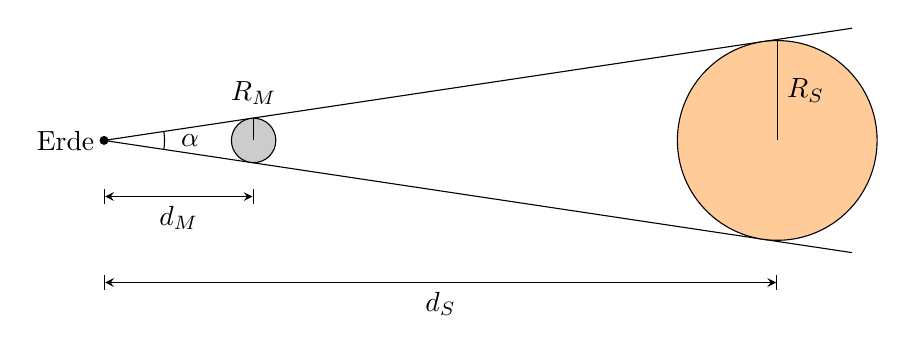
\begin{tikzpicture}[>=stealth, scale=0.95]
 \draw (0,0) -- (10,1.5);
 \draw (0,0) -- (10,-1.5);
 \fill (0,0) circle (0.06) node[left] {Erde};
 \draw[fill=gray!40] (2,0) circle (0.297);
 \draw[fill=orange!40] (9,0) circle (1.335);
 \draw (2,0) -- (2,0.297);
 \draw (9,0) -- (9,1.335) node[midway, right] {$R_\text{S}$};
 \node[above] at (2,0.35) {$R_\text{M}$};
 \draw (0.8,-0.12) arc (-8.53:8.53:0.8);
 \node at (1.15,0) {$\alpha$};
 \draw[|<->|] (0,-0.75) -- (2,-0.75) node[midway, below] {$d_\text{M}$};
 \draw[|<->|] (0,-1.9) -- (9,-1.9) node[midway, below] {$d_\text{S}$};
\end{tikzpicture}
\end{center}

Die beiden Scheiben füllen denselben Sehwinkel $\alpha$ aus. Für kleine Winkel ist
\begin{align}
 \frac{\alpha}{2} &\approx \frac{R_\text{M}}{d_\text{M}} = \frac{R_\text{S}}{d_\text{S}}
 \quad\Rightarrow\quad \frac{R_\text{S}}{R_\text{M}} = \frac{d_\text{S}}{d_\text{M}}
\end{align}
Die Radien \result{\text{verhalten sich wie die Abstände}} von der Erde. Mit den mittleren Entfernungen $d_\text{M} = \dMoO$ und $d_\text{S} = \dSoO$ (FoTaBe S.~210 und 211):
\begin{align}
 \frac{R_\text{S}}{R_\text{M}} &= \qdF = \frac{\dSo}{\dMo} = \qd \approx \result{\qdP{0}{2}}
\end{align}
Die Sonne ist also rund vierhundertmal so weit entfernt und rund vierhundertmal so gross wie der Mond. Die Radien aus der Formelsammlung bestätigen das: $R_\text{S}/R_\text{M} = \RSoO/\RMoO = \qRP{0}{2}$.
